\documentclass[conference,a4paper]{IEEEtran}
\usepackage{cite}
\usepackage{amsmath}
\usepackage{graphicx}
\usepackage{textcomp}
\usepackage{booktabs}
\usepackage{array}
\usepackage{url}
\usepackage{enumitem}
\setlist{itemsep=1pt,topsep=3pt,parsep=0pt}

\begin{document}

\title{Browser-Execution-Aware Detection of Command-and-Control Beacons Under Leakage-Free Evaluation}

\author{
\IEEEauthorblockN{L. K. Wadduwage, Hansika Mahaadikara, Amila Senarathne}
\IEEEauthorblockA{Department of Computer Systems Engineering\\
Sri Lanka Institute of Information Technology, Malabe, Sri Lanka\\
it22208408@my.sliit.lk, hansika.m@sliit.lk, amila.s@sliit.lk}
}

\maketitle

\begin{abstract}
A browser extension or a compromised web page that beacons to a command-and-control (C2) server produces periodic HTTPS requests that are indistinguishable from ordinary browsing at the network-flow level. This paper presents a detector that observes outbound requests inside a managed browser through the DevTools Protocol, labels each request with browser-execution context that no network capture can supply -- user activity, tab visibility, and request initiator -- and fuses a calibrated gradient-boosted classifier with nine deterministic rules. The principal contribution is methodological. Evaluating by unseen malware family and by unseen C2 infrastructure, rather than by a random split, exposed two defects in the training corpus: one family's positive windows were 95\% drawn from a single communicating pair, and that same capture was a non-periodic dead-server retry storm labelled as a beacon. Both defects are diagnosed, a scope criterion independent of the timing features used for detection is defined, and a threshold-placement bug introduced by probability calibration is corrected. On the corrected corpus, under one reliability rule applied uniformly to both protocols, the model reaches 92.3\% accuracy and 0.978 ROC-AUC on unseen C2 infrastructure and 83.8\% accuracy and 0.927 ROC-AUC on an unseen malware family, class-balanced and leakage-free.
\end{abstract}

\begin{IEEEkeywords}
command-and-control detection, browser security, dataset leakage, probability calibration, behavioral anomaly detection
\end{IEEEkeywords}

\section{Introduction}\label{sec:intro}

Command-and-control beaconing is the step that turns a compromise into an operation: the implant contacts its server on a schedule, receives instructions, and returns results. Detection has traditionally been treated as a network problem and solved by looking for regularity -- consistent inter-arrival times, consistent payload sizes, and a destination contacted at a cadence no human would produce \cite{garcia2014ctu13, gu2008botminer, bilge2012disclosure}. Beaconing is a named and persistent adversary technique in attack frameworks \cite{mitre2018attack}, and malicious browser extensions remain an active and growing threat class \cite{singh2025malicious}.

When beaconing moves inside the browser -- through a malicious extension, or script injected into a compromised page -- the network view degrades. The beacon's requests share the host's own TLS session with genuine browsing to the same destination, so a beacon to a chat platform or document service is indistinguishable at the flow level from a user with that service open. Encryption removes the payload, and flow-level defences must fall back on side-channel features to compensate \cite{anderson2016identifying}. What the network cannot see, the browser can: whether the user was interacting with the machine when a request fired, whether the tab was in the foreground, and whether an extension rather than a page initiated the request. This paper presents a browser-execution-aware detector built around that observation.

The principal contribution, however, is not the architecture but what happened when it was evaluated rigorously. A classifier trained on a real, published botnet capture produced strong held-out numbers under a random train/test split. Evaluating the same model with the malware family or specific attacker infrastructure held out entirely -- the only protocol that reflects what a deployed detector actually faces -- reduced those numbers sharply and forced a search for the cause. Two distinct corpus defects were found, rather than a modelling failure, together with a bug specific to the calibration step added to correct one of them. Concretely, this paper contributes:

\begin{itemize}
\item A non-invasive, browser-execution-aware collector on the Chrome DevTools Protocol producing a 29-feature per-host vector: 18 scale-free features read by the classifier, and 11 context or absolute-scale signals driving a deterministic heuristic layer, fused with fixed, measured weights (Section~\ref{sec:method}).
\item Diagnosis and correction of \emph{pseudo-replication} -- one family's positive windows were 95\% drawn from a single communicating pair -- and of an \emph{out-of-scope concept}, a non-periodic dead-C2 retry storm, removed by a scope criterion independent of the timing features used for detection (Section~\ref{sec:pseudorep}, Section~\ref{sec:outofscope}).
\item A threshold-placement bug specific to isotonic calibration, where a naive quantile rule is invalidated by calibration's tied outputs, isolated by ablation (Section~\ref{sec:calibration}).
\item Leakage-free evaluation by unseen family and unseen C2 source under one reliability rule, alongside a five-classifier comparison showing \emph{why} the deployed classifier was selected: an alternative wins the optimistic split and generalises to zero (Section~\ref{sec:results}).
\item A measured structural result: with fixed fusion weights, confirmed detection is unreachable from the learned signal alone once browser context is unavailable, a property of the architecture, not an artefact of training (Section~\ref{sec:fusionlimit}).
\end{itemize}

\section{Literature Review}\label{sec:litreview}

\subsection{Flow-Based Detection}
Regularity statistics over inter-arrival times, payload-size consistency, and destination entropy underpin most beacon detectors. The CTU-13 capture set \cite{garcia2014ctu13} remains a standard labelled corpus for this line of work; Gu \emph{et al.} cluster communication and activity patterns independently of protocol \cite{gu2008botminer}, and Bilge \emph{et al.} identify C2 servers from NetFlow records at scale \cite{bilge2012disclosure}. More recent work decodes beaconing periodicity directly for threat hunting \cite{mahboubi2025lurking}. None of this literature has browser execution context available to it, by construction: it operates on network captures.

\subsection{Browser-Mediated Threats}
Malicious browser extensions are an active and growing category, and recent large-scale studies characterise their behaviour and prevalence \cite{singh2025malicious}. Attributing traffic to a specific extension, tab, or script -- rather than to a page's own first-party traffic -- is not a property that flow-level tooling can recover, which motivates instrumenting the browser directly.

\subsection{Learning Under Scarce, Skewed Positives}
Isolation Forest \cite{liu2008isolationforest} targets settings where labelled anomalies are scarce relative to abundant normal traffic. Gradient-boosted trees such as XGBoost \cite{chen2016xgboost} are the supervised alternative once sufficient positives exist, but require explicit correction of their predicted probabilities: margin-based ensembles push scores away from 0 and 1, a distortion Niculescu-Mizil and Caruana correct with isotonic regression \cite{niculescumizil2005predicting}, which motivates the calibration step in Section~\ref{sec:calibration}.

\subsection{Evaluation Bias}
Random or otherwise leakage-permissive splits over a corpus assembled from few sources overstate held-out performance. Sommer and Paxson argue that closed-world machine-learning evaluation transfers poorly to intrusion detection \cite{sommer2010outside}; Pendlebury \emph{et al.} formalise this for malware classification across space and time \cite{pendlebury2019tesseract}, and Arp \emph{et al.} catalogue recurring pitfalls -- sampling bias, spurious correlations, inappropriate measures -- across three decades of security-ML papers \cite{arp2022dos}. The leave-one-family-out and leave-one-C2-source-out protocols used here apply that principle to a beacon corpus built from grouped, windowed captures; the pseudo-replication defect in Section~\ref{sec:pseudorep} is a concrete instance of the sampling bias these authors describe.

\subsection{Research Gap}
The literature above establishes methods for flow-level regularity detection, documents browser extensions as a growing threat surface, and warns that evaluation protocol determines whether reported accuracy is credible. No prior work combines all three: a browser-execution-aware detector evaluated under a grouped, leakage-controlled protocol, with the corpus itself audited for pseudo-replication and label-concept scope. That combination is the gap this paper addresses.

\section{Methodology}\label{sec:method}

\begin{figure*}[t]
\centering
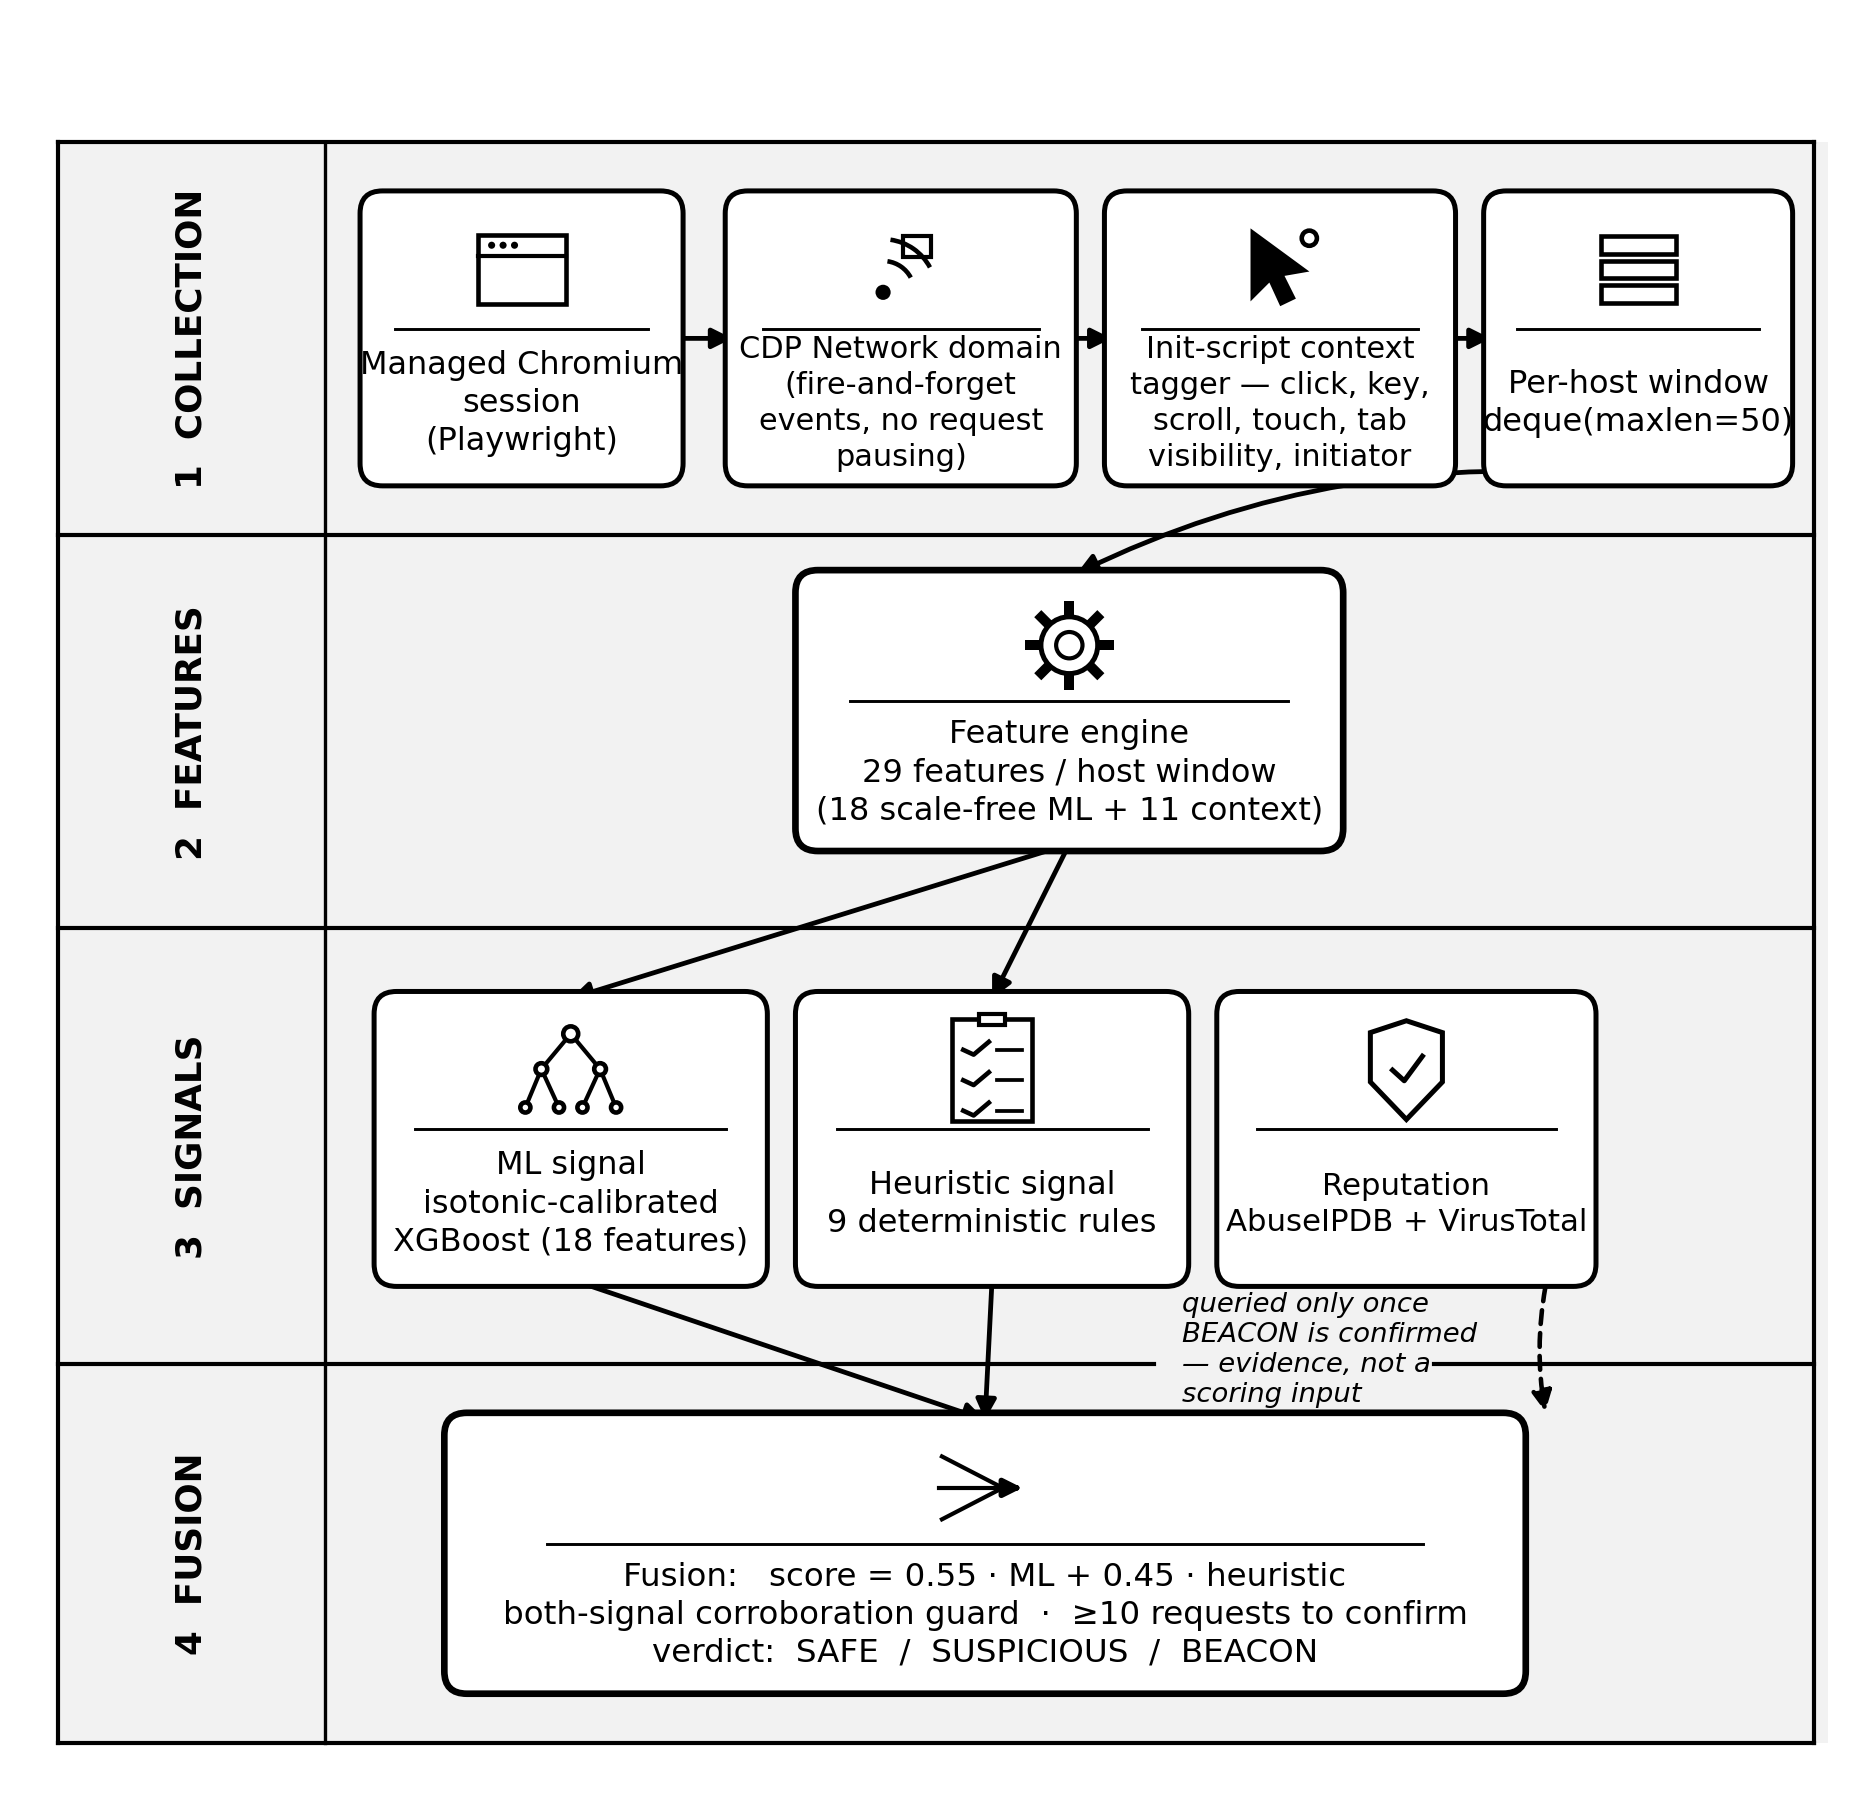
\includegraphics[width=0.86\textwidth]{figures/fig1_architecture.png}
\caption{The detection pipeline. Analysis runs every 10 seconds for each monitored destination host. Reputation is consulted only after a confirmed detection and is never an input to the score.}
\label{fig:arch}
\end{figure*}

\subsection{Non-Invasive Collection}
Requests are captured through the Network domain of the DevTools Protocol rather than through request interception (Fig.~\ref{fig:arch}). This is a performance decision: protocol events are fire-and-forget, so the browser never waits on the analysis process, whereas a global route handler pauses every outgoing request until it responds \cite{chromedevtools, playwright}, a real cost on any page issuing many concurrent requests. User interaction (click, keydown, scroll, touchstart) and tab visibility are recorded by an init script. Pointer movement is deliberately excluded, since it fires from passive cursor presence and inflates measured activity for exactly the two features that matter most. Requests from service workers and other non-page contexts are attributed to the background with the user marked inactive.

\subsection{Feature Vector}
Every 10 seconds, the rolling window of up to 50 requests per destination host -- a fixed-size deque from which the oldest requests are dropped -- is reduced to 29 features. Eighteen are scale-free (ratios, shares, normalised entropies) and are the only features the classifier reads (Table \ref{tab:features}); absolute byte counts or intervals were found to teach the model the scale of a 2011 capture rather than the property of beaconing (Section~\ref{sec:datasetconstruction}). The most important trained feature, at 31.8\% of total gain, is not a timing statistic: it is the share of requests carrying no \texttt{Referer} header, since a timer-fired request is not the result of a click. The remaining 11 features (inter-arrival mean and MAD, burst count, requests per hour, same-site ratio, script-initiator ratio, four context fields) drive the heuristic layer directly -- absolute-scale or context features no offline network corpus can label.

\begin{table}[t]
\caption{The 18 scale-free ML features, by group, with trained importance}
\label{tab:features}
\centering
\small
\setlength{\tabcolsep}{3pt}
\begin{tabular}{p{0.20\columnwidth}p{0.58\columnwidth}c}
\toprule
\textbf{Group} & \textbf{Features} & \textbf{Imp.} \\
\midrule
Timing shape (8) & inter-arrival CV, Bowley skewness, normalized MAD, burstiness, lag-1 autocorrelation, spread ratio, clock-boundary share, normalized entropy & 29.8\% \\
Payload size (4) & mean, coefficient of variation, size-repeat ratio, upload/download ratio & 19.6\% \\
URL / method (5) & path entropy, unique-path ratio, POST ratio, normalized URI length, URI character entropy & 18.8\% \\
Request behaviour (1) & Referer-absent ratio & \textbf{31.8\%} \\
\bottomrule
\end{tabular}
\end{table}

\subsection{Heuristic Layer and Fusion}\label{sec:heuristic}
Nine deterministic rules score, in turn: regular timing with a small payload; foreground requests firing during long user idle periods; background-tab traffic; extension-origin foreground beacon shape; low path entropy with regular timing and inactivity; script-initiated regularity; a high POST ratio with regular timing; a sustained high request rate while inactive; and, last and only multiplicatively, a same-site dampener that reduces -- never raises -- suspicion for traffic to the active page's own site, so legitimate single-page-application background sync is not mistaken for a beacon.

The fused score is a fixed weighted sum, \(\mathrm{score} = 0.55 \cdot \mathrm{ML} + 0.45 \cdot \mathrm{heuristic}\), mapped to SAFE ($<0.30$), SUSPICIOUS ($<0.52$), or BEACON ($\geq 0.52$); Section~\ref{sec:fusionlimit} reports how the weight was chosen. A both-signal corroboration guard withholds a BEACON verdict whenever either signal falls below a low floor, so a verdict never rests on one signal alone. A hard floor requires at least 10 observed requests before BEACON can be confirmed, and timing-dependent signals ramp in between 6 and 20 requests rather than switching on at a hard cutoff. Reputation services (AbuseIPDB, VirusTotal) are queried only after a BEACON verdict is confirmed, results cached for 30 minutes as supporting evidence; reputation is never an input to the fused score.

\subsection{Dataset Construction}\label{sec:datasetconstruction}
The training corpus consists exclusively of real HTTP request records derived from public botnet captures, windowed into consecutive, non-overlapping blocks of real requests for each communicating pair. No row is synthetic. Before the corrections described below, the corpus contained 68{,}464 windows across six malware families, of which 6{,}890 were positive.

\subsection{Pseudo-Replication}\label{sec:pseudorep}
One family contributed 6{,}551 of those 6{,}890 positive windows (95.1\%), but every one came from a single \((\mathrm{src}, \mathrm{dst})\) pair: one infected host, one C2 server, one continuous session cut into blocks. Counted by independent communicating pair rather than window, that family is 1 of 53, or 1.9\%: a window count over a corpus built by slicing continuous sessions overstates the independent evidence available. This is a concrete instance of the sampling bias described in \cite{arp2022dos, pendlebury2019tesseract}, invisible to any evaluation that shuffles windows.

\subsection{Out-of-Scope Concept}\label{sec:outofscope}
The same dominant capture is a dead C2: the server was unreachable and the malware was retrying into HTTP error responses. Its timing is retry backoff rather than a scheduled beacon (Table \ref{tab:scope}), indistinguishable from ordinary browsing on the regularity feature the detector depends on most, and inverted relative to every other family on URI character entropy. Training on it forced the model to reconcile two different generative processes under a single label.

\begin{table}[t]
\caption{Feature medians, C2 windows only: the excluded capture is not periodic}
\label{tab:scope}
\centering
\small
\begin{tabular}{lccc}
\toprule
\textbf{Feature} & \textbf{Excluded} & \textbf{Other C2} & \textbf{Benign} \\
\midrule
Inter-arrival CV$\downarrow$ & 1.613 & 0.005 & 1.909 \\
Clock-boundary share$\uparrow$ & 0.082 & 1.000 & 0.095 \\
Error-response ratio & 1.000 & 0.043 & 0.267 \\
\bottomrule
\end{tabular}
\end{table}

\subsection{Scope Criterion and Cap}\label{sec:scope}
To avoid circularity with the timing features used for detection, scope is defined on channel outcome rather than on timing: a C2 window is in scope only if its error-response ratio is below 1.0, meaning the channel completed at least one successful exchange. A per-pair cap of 150 windows bounds the contribution of any single session. The resulting corpus contains 55{,}844 windows, of which 330 are positive, drawn from 50 independent C2 pairs across six families, and is used for training and for every evaluation result in Section~\ref{sec:results}.

Excluding the dead-C2 traffic from training did not remove the ability to detect it: scored against benign windows held out of training, it is caught 100\% of the time at the deployed threshold, with ROC-AUC 0.995 against those negatives. Adding the error-response ratio as a nineteenth ML feature was considered and rejected: it separates the excluded capture almost perfectly (median 1.000) but sits on the \emph{opposite} side of benign traffic for every other C2 family (0.043), so it would teach the model that the server is down rather than that the traffic is a beacon.

\subsection{Classifier and Training}
The classifier is XGBoost \cite{chen2016xgboost} with monotone constraints encoding directional domain priors -- for example, the predicted probability may only decrease as the inter-arrival coefficient of variation rises. It is fitted with per-row sample weights that equalise the training contribution of each malware family and equalise real browsing against lab-background benign traffic: re-weighting rather than resampling, so no window is duplicated or invented.

\subsection{Calibration and Threshold Placement}\label{sec:calibration}
Motivated by the finding that boosted-tree probabilities are systematically distorted \cite{niculescumizil2005predicting}, the model is wrapped in isotonic calibration with grouped inner cross-validation, implemented with scikit-learn \cite{pedregosa2011scikit}. The decision threshold is placed at a target false-positive rate measured on benign traffic -- the \((1-\mathrm{fpr})\) quantile of the benign score distribution -- with the target FPR chosen by inner grouped cross-validation on training data only, mirroring how a deployed sensor is tuned against its own environment's benign traffic, using no attack labels.

A threshold-placement bug was found and fixed here. The first implementation placed this threshold with \texttt{numpy.quantile}, but isotonic regression's output is a step function with heavy ties, so that quantile routinely lands on a value shared by many benign windows, and \(\mathrm{score} \geq \mathrm{threshold}\) then admits all of them at once. A fold with ROC-AUC 0.927, with ranking clearly intact, produced a precision inconsistent with any real operating point because the false-positive budget had been silently exceeded. The rule was replaced with a tie-aware ascending scan for the smallest threshold whose \emph{achieved} FPR on held-out benign traffic meets the budget. Changing only this rule, leave-one-family-out F1 moves from 0.7635 to 0.8289 while ROC-AUC is unchanged at 0.9266, confirming the bug affected threshold placement and not ranking.

\subsection{Evaluation Protocol}\label{sec:protocol}
Test sets are class-balanced -- benign windows are subsampled to the positive count, and five independent draws are averaged -- so accuracy and precision are meaningful rather than a restatement of a sub-1\% prevalence. Decision thresholds are always chosen by inner grouped cross-validation on training data only, never on the fold being scored. Two held-out protocols are reported: \textbf{LOPO} (leave-one-C2-source-out), holding out one communicating pair at a time, representing a known family reaching new infrastructure; and \textbf{LOFO} (leave-one-malware-family-out), holding out an entire family, representing one never seen in training.

One reliability rule applies uniformly to both: a fold contributes to a reported mean only if it contains at least ten positive test windows, since three positives cannot distinguish a working detector from a fortunate one. Of the 50 in-scope C2 pairs, 15 form a LOPO fold at all, and four clear the ten-positive bar; of six malware families, three clear it. All means in Section~\ref{sec:results} are taken over those folds only.

\section{Results and Discussion}\label{sec:results}

\begin{figure}[t]
\centering
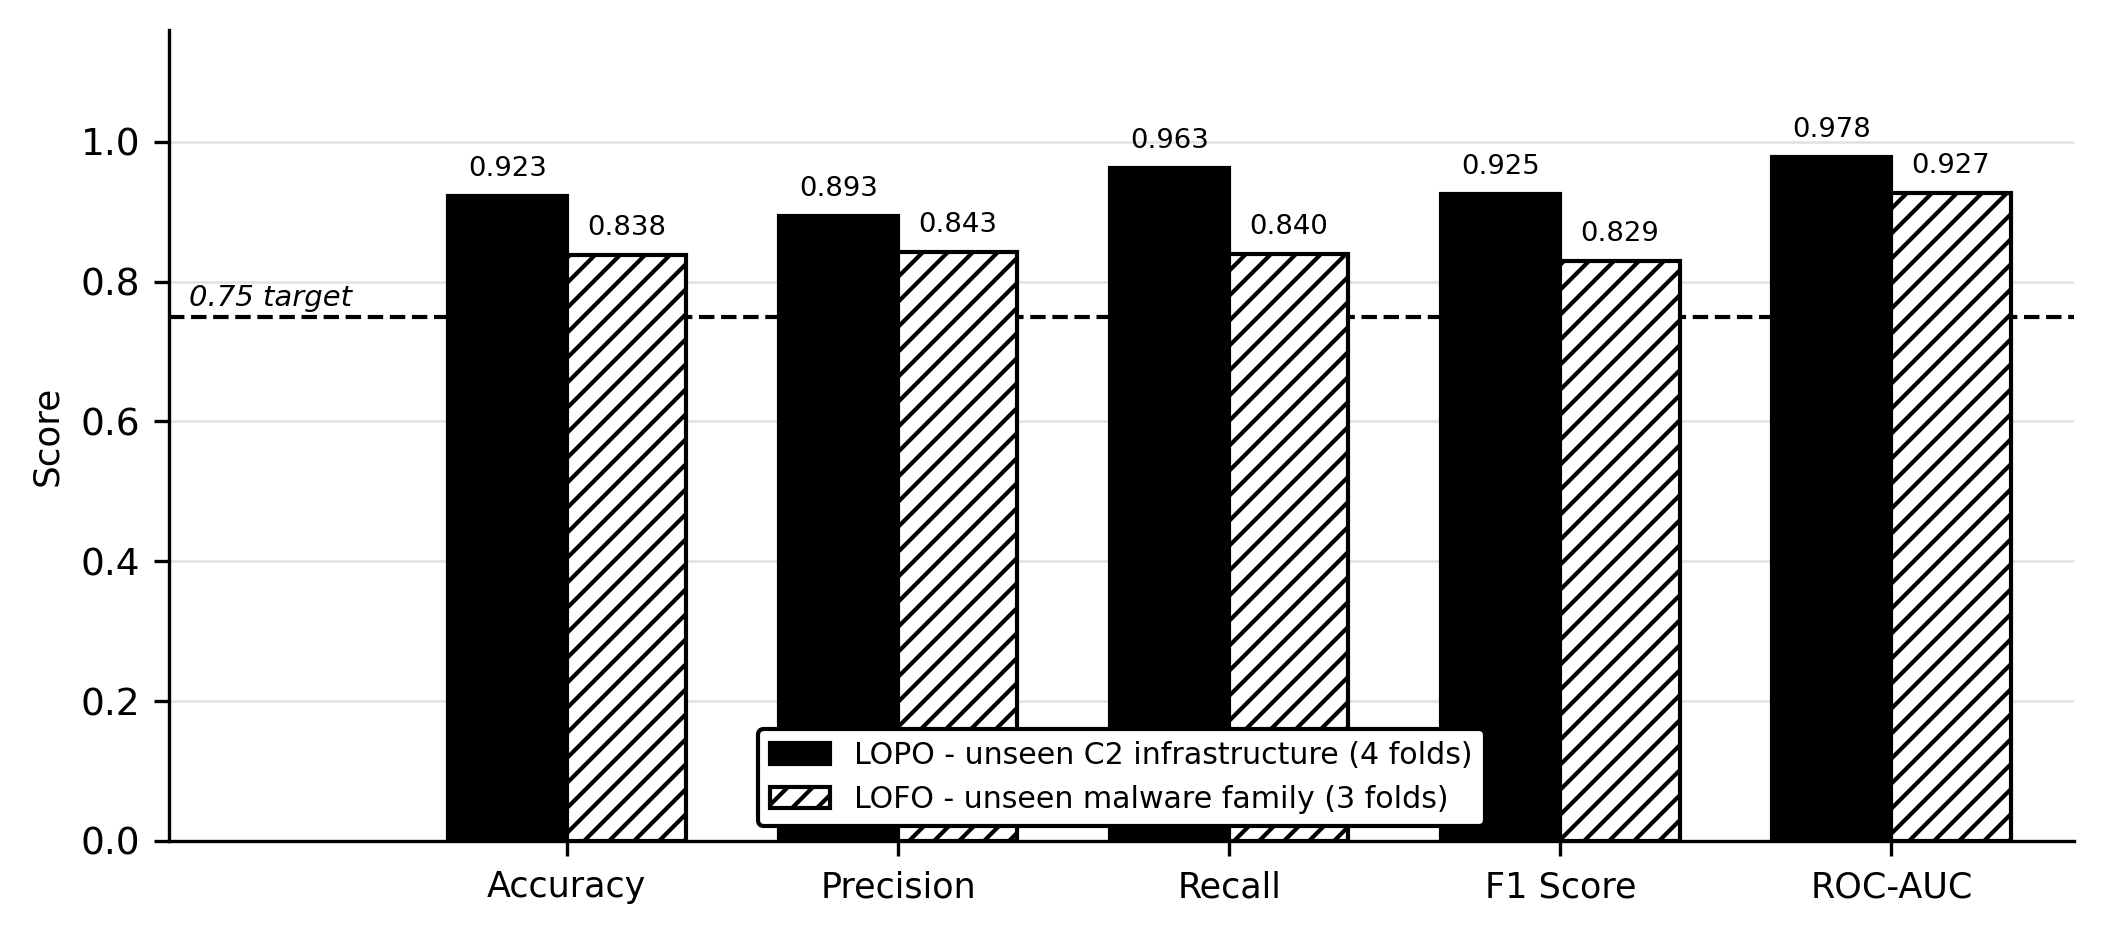
\includegraphics[width=\columnwidth]{figures/fig2_headline_results.png}
\caption{Class-balanced held-out performance of the deployed model. Both protocols apply the same reliability rule: a fold enters a mean only if it contains at least ten positive test windows.}
\label{fig:headline}
\end{figure}

\subsection{Headline Results}\label{sec:headline}
Table \ref{tab:headline} and Fig.~\ref{fig:headline} report both protocols for the deployed model. Every reported mean exceeds the 0.75 target on every metric, but two qualifications matter.

First, applying the reliability rule to LOPO is not a cosmetic choice: averaging all 15 pair folds instead -- including 11 that contain only three positive windows each, on which the model is trivially correct -- would report 96.2\% accuracy and 0.991 ROC-AUC, visibly higher on every metric. That figure is listed in Table \ref{tab:headline} for transparency but is regarded as inflated by folds too small to carry information, and is not claimed.

Second, the mean is not the whole story: one held-out family, ZeusV1, reaches only 60.2\% recall and 71.1\% F1, below target, even though it does not pull the three-family mean below it. ZeusV1 is also the largest held-out family, contributing 226 of the 330 in-scope positive windows across three distinct C2 servers, so it is the best-supported single measurement in the LOFO set rather than a small-sample outlier, and is reported rather than averaged away.

\begin{table}[t]
\caption{Deployed model, class-balanced held-out evaluation. LOPO holds out one C2 source; LOFO holds out an entire malware family. Means cover only folds with at least ten positive test windows; the final row is shown for transparency and is not claimed.}
\label{tab:headline}
\centering
\footnotesize
\setlength{\tabcolsep}{3.4pt}
\begin{tabular}{lccccc}
\toprule
\textbf{Protocol} & \textbf{Acc.} & \textbf{Prec.} & \textbf{Rec.} & \textbf{F1} & \textbf{AUC} \\
\midrule
LOPO (4 folds) & 92.3\% & 89.3\% & 96.2\% & 92.5\% & 0.978 \\
LOFO (3 folds) & 83.8\% & 84.3\% & 84.0\% & 82.9\% & 0.927 \\
\midrule
\quad ZeusV1 fold only & 75.5\% & 86.9\% & 60.2\% & 71.1\% & 0.887 \\
\quad LOPO, all 15 folds & 96.2\% & 94.8\% & 99.0\% & 96.6\% & 0.991 \\
\bottomrule
\end{tabular}
\end{table}

\subsection{Why the Gradient-Boosted Classifier Was Selected: A Five-Classifier Comparison}\label{sec:classifiercomp}
Logistic regression, Naive Bayes, a decision tree, Random Forest, and XGBoost were trained on the identical scoped corpus, with identical features and sample weights, and no per-model threshold tuning: a fixed 0.5 threshold at natural prevalence. This is a different, uncalibrated protocol from Table \ref{tab:headline}, included only to justify the architecture choice. Table \ref{tab:classifiers} and Fig.~\ref{fig:classifiers} report the result. Random Forest wins the optimistic grouped split (F1 0.688, AUC 0.996) and then predicts \emph{zero} positives on every held-out family: precision, recall, and F1 are exactly 0.000 across all six families, despite a still-informative ROC-AUC of 0.740 -- its ranking survives the family shift, but no unseen-family window ever crosses 0.5. The split AUC of Naive Bayes (0.467, worse than chance) reflects its independence assumption being violated by strongly correlated timing features. XGBoost has both the best LOFO ROC-AUC (0.858) and the best LOFO F1 (0.267) of the five, the basis for its selection: cross-family ranking rather than in-distribution accuracy.

\begin{figure}[t]
\centering
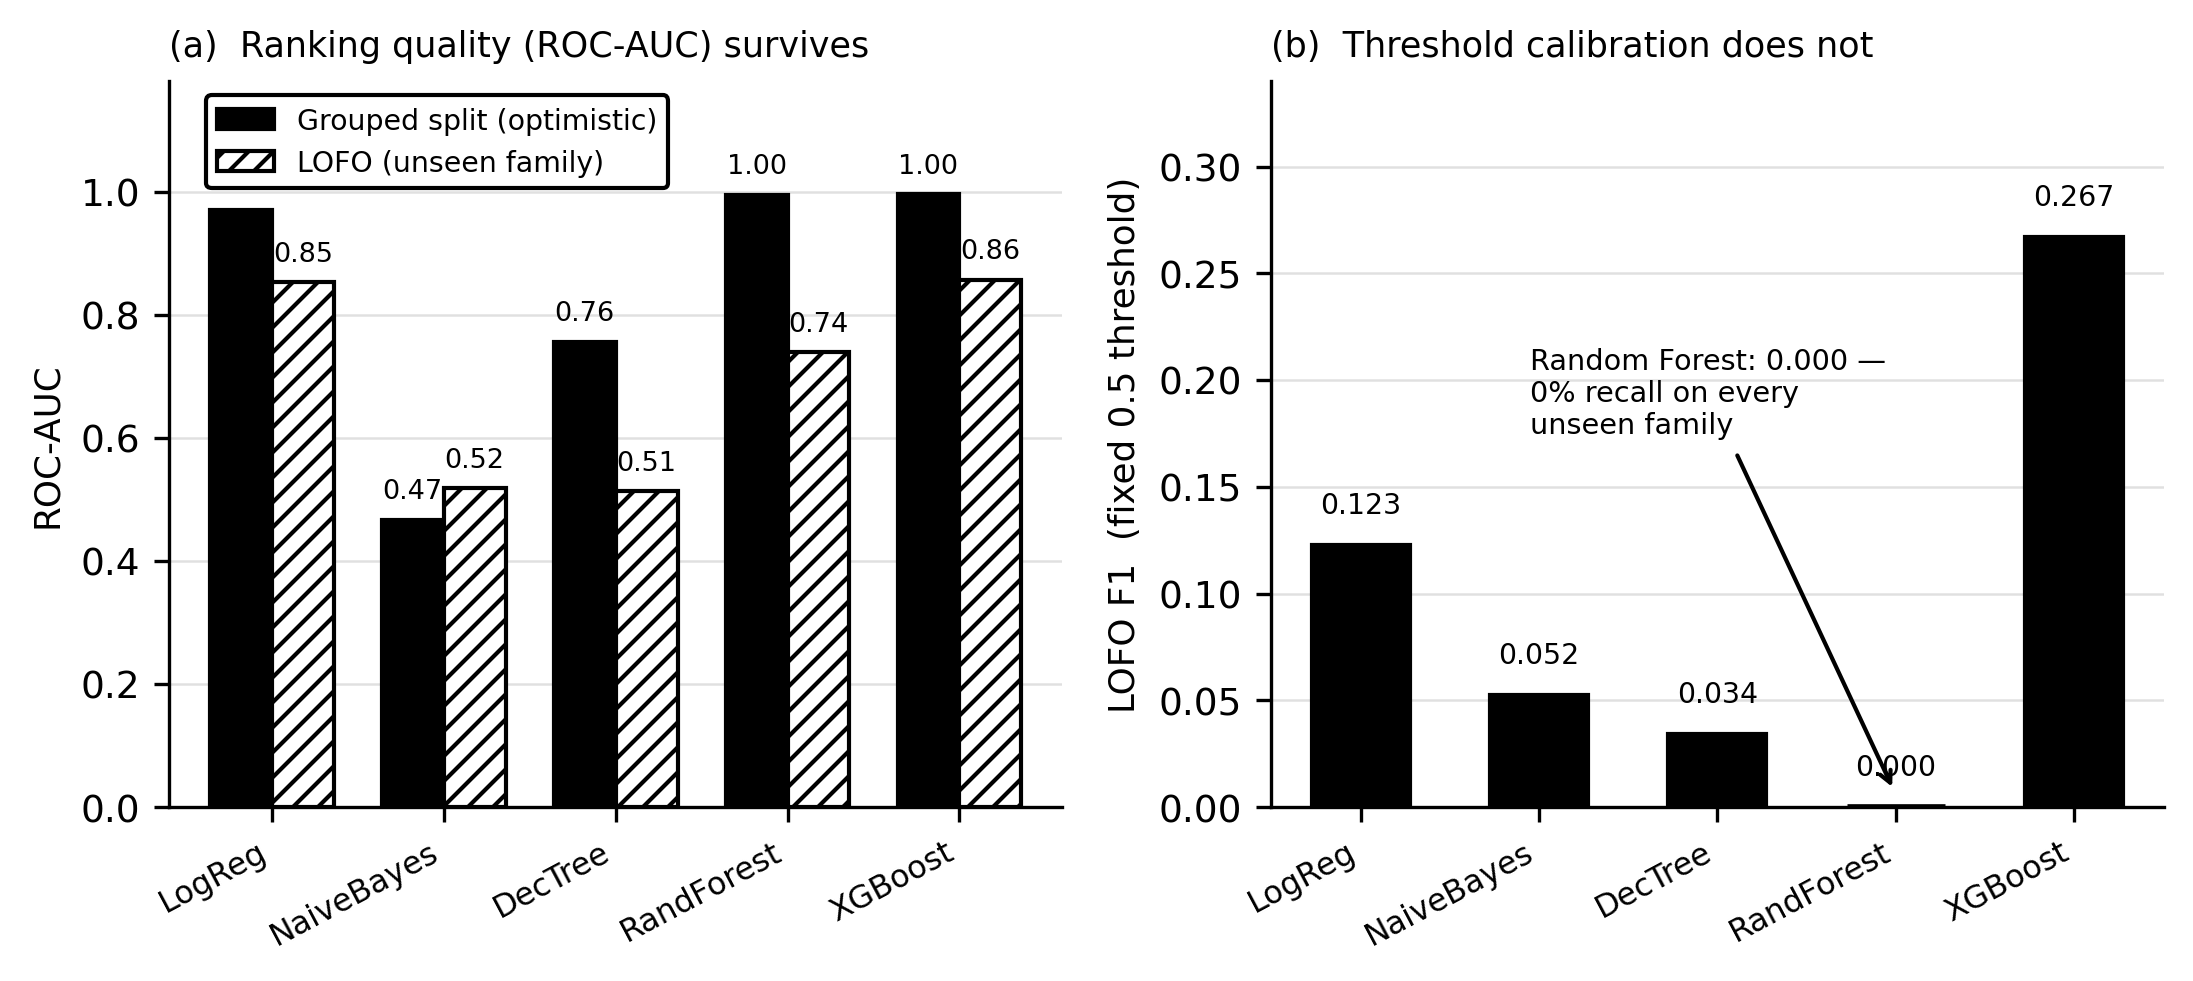
\includegraphics[width=\columnwidth]{figures/fig3_classifier_comparison.png}
\caption{Five classifiers on the identical scoped dataset and weighting. Random Forest wins the optimistic split, then fails to generalise: ranking quality partly survives an unseen family, but calibration to a fixed threshold does not.}
\label{fig:classifiers}
\end{figure}

\begin{table}[t]
\caption{Five classifiers, identical scoped data, fixed 0.5 threshold}
\label{tab:classifiers}
\centering
\small
\begin{tabular}{lccc}
\toprule
\textbf{Classifier} & \textbf{Split F1} & \textbf{LOFO F1} & \textbf{LOFO AUC} \\
\midrule
Logistic Regression & 0.096 & 0.123 & 0.853 \\
Naive Bayes & 0.024 & 0.052 & 0.518 \\
Decision Tree & 0.640 & 0.034 & 0.514 \\
Random Forest & \textbf{0.688} & 0.000 & 0.740 \\
XGBoost (deployed) & 0.452 & \textbf{0.267} & \textbf{0.858} \\
\bottomrule
\end{tabular}
\end{table}

\subsection{Fusion Weight and a Structural Limit}\label{sec:fusionlimit}
The ML weight was swept from 0.45 to 0.70 through the real fusion function on the full scoped corpus, under an assumed idle-background browser context. BEACON F1 peaks at weight 0.55 (0.9745, against 0.9324 at 0.45); beyond 0.55, precision falls faster than recall rises. This is the weight deployed in Section~\ref{sec:heuristic}.

Separately, under a context-blind condition where no browser-context fields are available -- the most any network-only capture could ever supply -- confirmed-BEACON recall measures \textbf{exactly 0.000 at every tested weight from 0.45 to 0.70}. This is not a training artefact: it follows from the both-signal corroboration guard withholding confirmation whenever the heuristic term sits at its floor, regardless of how the two weights are divided. SUSPICIOUS-tier detection is unaffected across the same range (F1 between 0.947 and 0.967), so nothing is silently missed; it surfaces at a lower confidence tier instead -- the central operational claim of this paper: no re-weighting of the fusion substitutes for the browser-execution context the architecture is built to supply.

\subsection{Discussion}
These results together show that measured accuracy on this task is highly sensitive to evaluation protocol: the same corpus and classifier report either 96\% or 84\% depending on which folds are averaged. This sensitivity is not unique to gradient boosting -- Random Forest's optimistic-split win does not predict its cross-family behaviour at all -- so protocol, not classifier choice alone, determines whether a reported number holds up against new attacker infrastructure. The structural fusion result indicates that no algorithmic tuning substitutes for the browser-execution context the architecture supplies; this is a design constraint, not a shortcoming to optimise away later.

\section{Limitations and Future Work}\label{sec:limitations}

\begin{itemize}
\item One held-out family, ZeusV1, falls below the 0.75 target on recall and F1, although the aggregate mean clears it (Section~\ref{sec:headline}). Because it is the largest held-out family, this is a real limit of cross-family generalisation rather than a sampling artefact.
\item Three of the six families are too small to evaluate meaningfully and are excluded from all reported means: Sogou and ZeusB26, with three held-out positive windows each, and Zeus78, which retains one window after the scope criterion is applied.
\item Detection scope is active, periodic C2. A channel that never completes an exchange lies outside the trained concept, although it is separately shown to remain detectable (Section~\ref{sec:scope}).
\item Confirmed BEACON detection architecturally requires corroborating browser context and is unreachable from the model alone without it (Section~\ref{sec:fusionlimit}), which is a limitation for any deployment that cannot instrument the browser.
\item The corpus predates modern jittered and malleable C2 frameworks. Extending coverage requires new labelled captures rather than further mining of the present ones.
\end{itemize}

Future work will extend the corpus to modern jittered and malleable C2 frameworks, which post-date the public captures used here and are known to defeat pure timing-regularity features, and will close the ZeusV1 gap (Section~\ref{sec:headline}) by collecting additional labelled infrastructure for that family rather than by re-tuning the existing model. The context-blind result (Section~\ref{sec:fusionlimit}) also motivates extending browser instrumentation to service workers, third-party iframes, and mobile DevTools Protocol variants, so the corroboration the fusion layer requires stays available across more deployments. Finally, connecting confirmed-BEACON verdicts to network-layer enforcement, such as an outbound firewall rule keyed to the flagged destination, would close the loop from detection to mitigation without a human in that step.

\section{Conclusion}\label{sec:conclusion}

Evaluating a browser-execution-aware C2 detector by unseen malware family and unseen infrastructure, rather than by a random split, did more than lower a number: it surfaced a pseudo-replicated training corpus, an out-of-scope traffic concept hiding inside the positive class, and a calibration-specific threshold bug, each diagnosed from first principles and corrected. Applying one reliability rule uniformly to both held-out protocols, the corrected model reaches 92.3\% accuracy on unseen infrastructure and 83.8\% on an unseen malware family, class-balanced and leakage-free; the higher figure a less careful aggregation would have produced is also reported and explicitly not claimed. A five-architecture comparison shows the deployed classifier was chosen for surviving family shift, not for winning an optimistic split, since the alternative that wins the split generalises to nothing. The paper closes with a structural limitation measured directly: no fusion weight recovers confirmed detection from the model alone once browser context is unavailable, restating the paper's central argument as an engineering fact.

\section*{Acknowledgment}
The authors thank the members of research group R26-CS-003 for their collaboration on the shared WebSentinel platform, and the Stratosphere Laboratory for the public captures on which this work depends.

\bibliographystyle{IEEEtran}
\bibliography{ICAC2026_BeaconDetector_references}

\end{document}
